\subsection{Insegnante}

\subsubsection{Panoramica insegnante}
\begin{figure}[H]
\centering
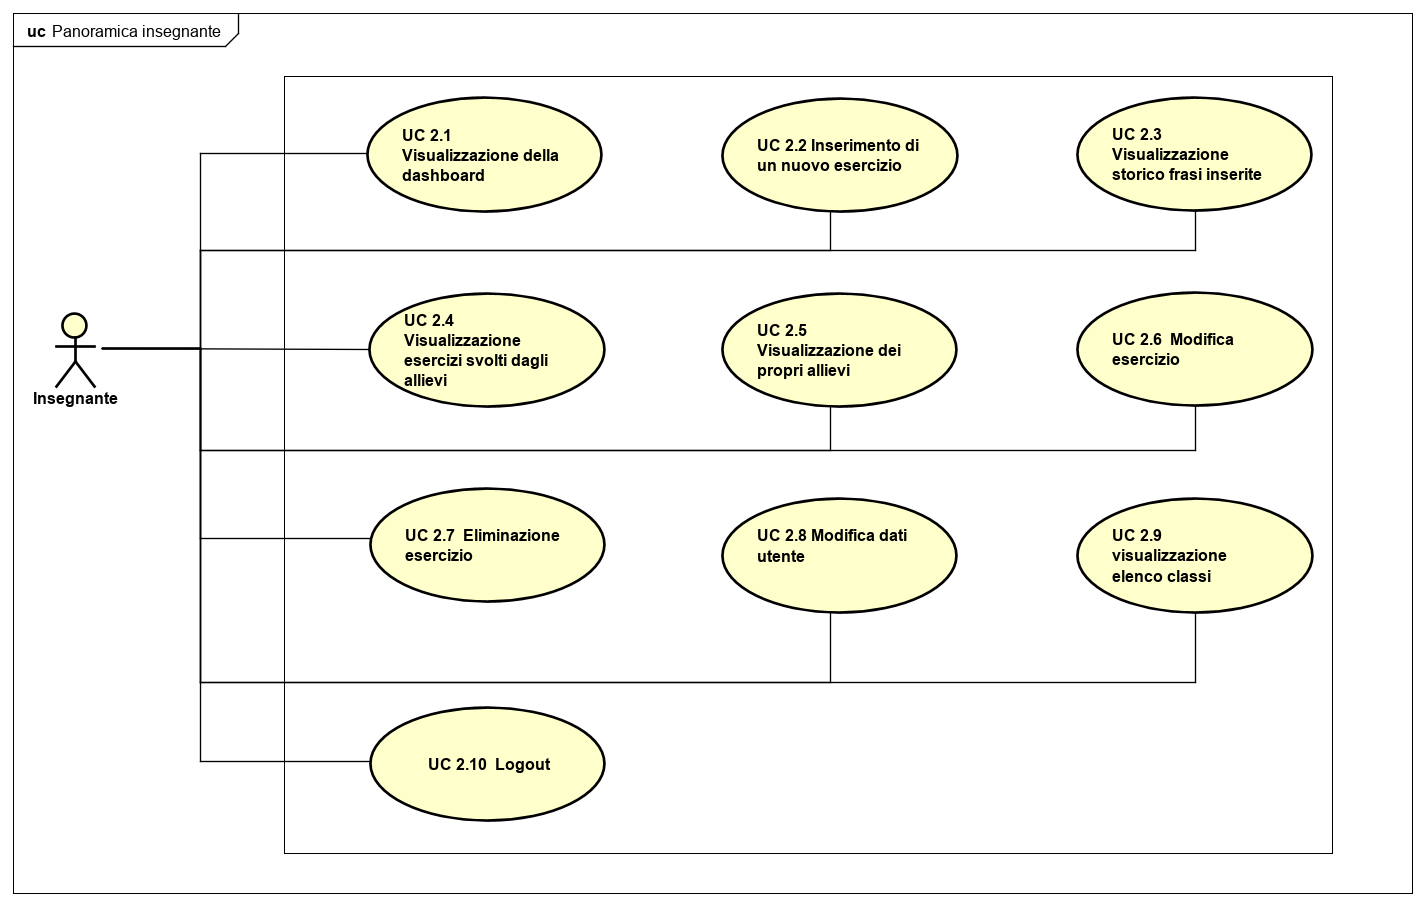
\includegraphics[width=17cm, height=20cm]{img/PanoramicaInsegnanti.png} 
\caption{Panoramica insegnante}
\end{figure}

\subsubsection{UC 2.1 Visualizzazione della dashboard}
\begin{itemize}
	\item[•] \textbf{Attori}: Insegnante;
	\item[•] \textbf{Descrizione}: l’insegnante accede alla propria dashboard;
	\item[•] \textbf{Precondizione}: l'insegnante si è autenticato;
	\item[•] \textbf{Postcondizione}: l'insegnante visualizza tutti i componentidella sua dashboard;
	\item[•] \textbf{Flusso degli eventi}: l’insegnante alla propria dashboard dove può vedere i suoi dati, le frasi che ha assegnato agli alunni, il numero e i nomi degli studenti che possiede e può effettuare modifiche agli esercizi.
\end{itemize}

\subsubsection{UC 2.2 Inserimento di un nuovo esercizio}
\begin{figure}[H]
	\centering
	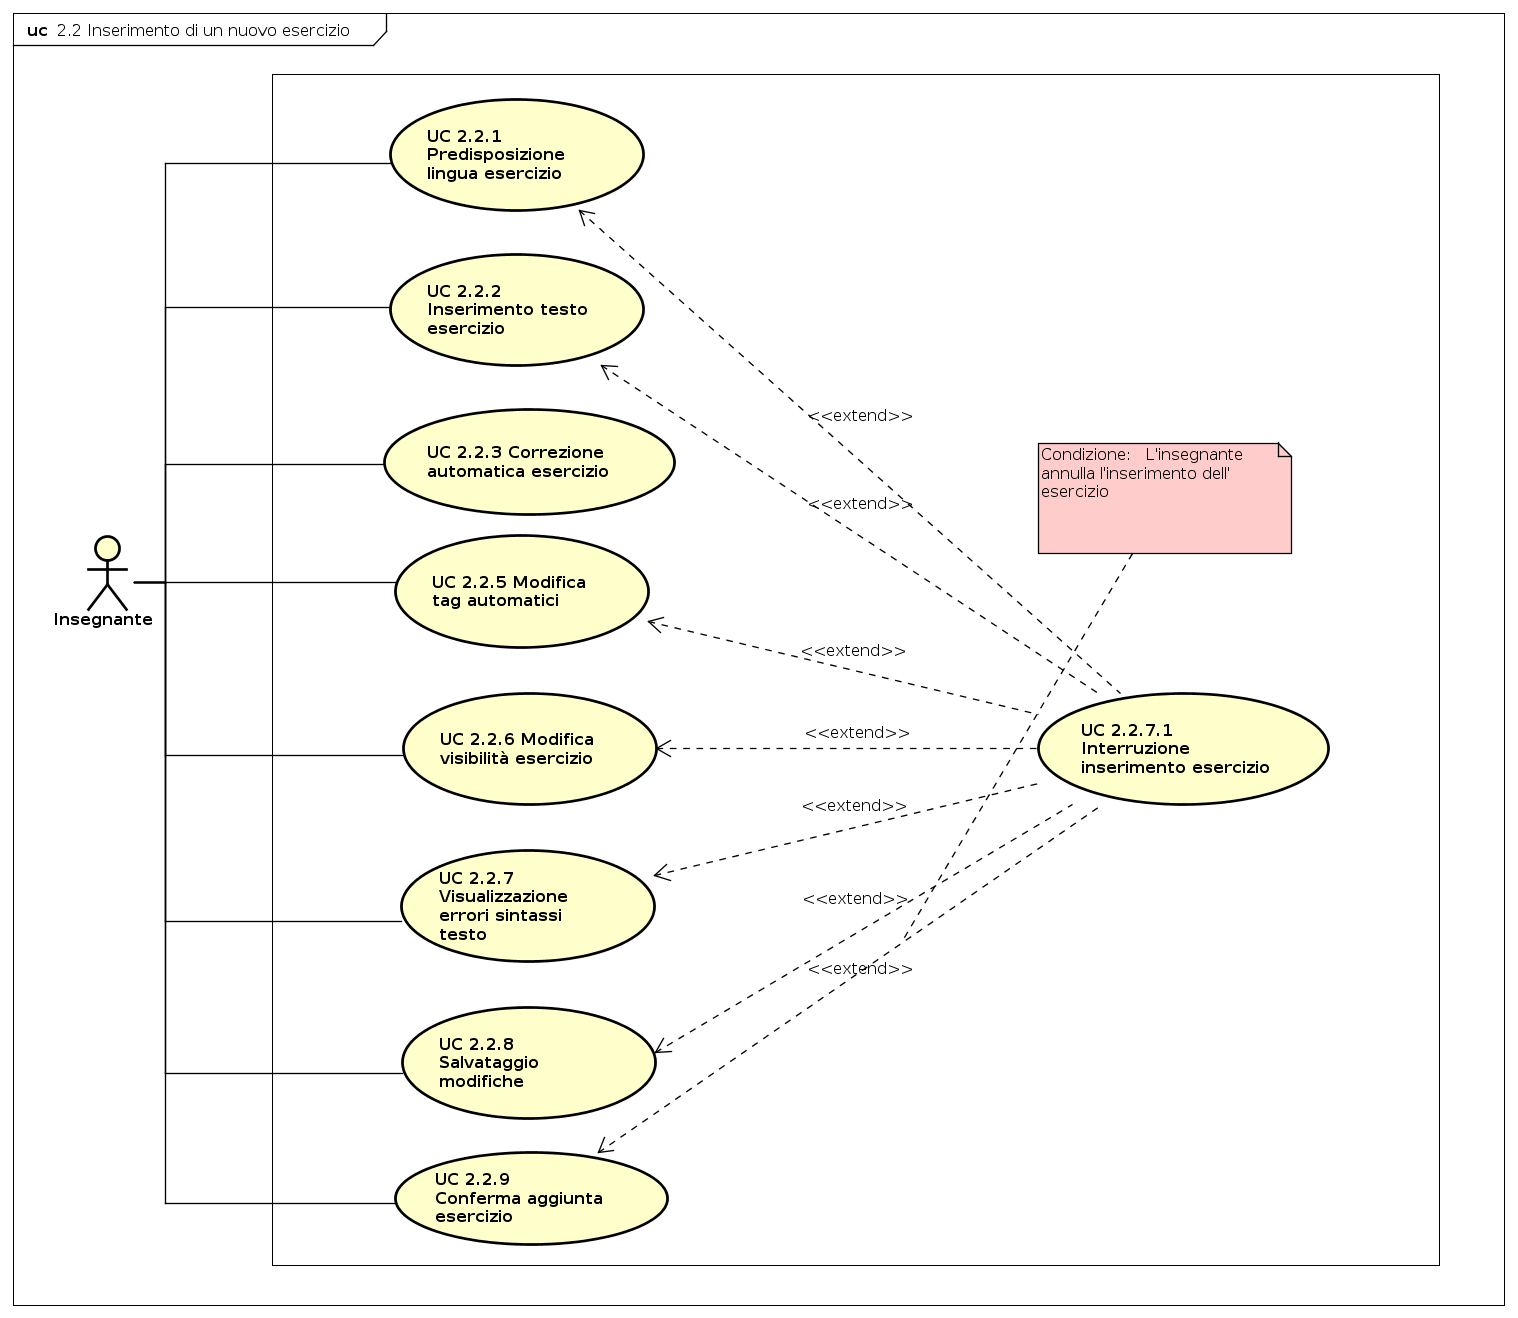
\includegraphics[width=17cm]{img/UC22.png} 
	\caption{Caso d'uso UC 2.2;}
\end{figure}


\begin{itemize}
	\item[•] \textbf{Attori}: Insegnante;
	\item[•] \textbf{Descrizione}: l'insegnante aggiunge un nuovo esercizio e può scegliere la lingua, scrivere il testo,
modificare i tag automatici ecc. Potrà poi confermare l'aggiunta dell'esercizio;
	\item[•] \textbf{Precondizione}: l'insegnante si è autenticato e visualizza la propria dashboard;
	\item[•] \textbf{Postcondizione}: l'insegnante ha inserito un esercizio;
	\item[•] \textbf{Flusso degli eventi}:
	\begin{enumerate}
		\item UC 2.2.1 Predisposizione lingua esercizio;
		\item UC 2.2.2 Inserimento testo esercizio;
		\item UC 3.10.3  Visualizzazione analisi automatica;
		\item UC 2.2.5 Modifica tag automatici;
		\item UC 2.2.6 Modifica visibilità esercizio;
		\item UC 2.2.7 Visualizzazione errori sintassi testo;
		\item UC 2.2.8 Salvataggio modifiche;
		\item UC 2.2.9 Conferma aggiunta esercizio.
	\end{enumerate}
	\item[•] \textbf{Estensioni}:	
	\begin{enumerate}
		\item UC 2.2.7.1 Interruzione inserimento esercizio.
	\end{enumerate}
	\item[•] \textbf{Flusso degli eventi alternativo}:
	\begin{enumerate}
		\item UC 2.2.4 Inserimento soluzione alternativa.
	\end{enumerate}
\end{itemize}

\subsubsection{UC 2.2.1 Predisposizione lingua esercizio}
\begin{itemize}
	\item[•] \textbf{Attori}: Insegnante;
	\item[•] \textbf{Descrizione}: l'insegnante sceglie la lingua dell’esercizio che vuole scrivere;
	\item[•] \textbf{Precondizione}: l'insegnante sta inserendo un esercizio;
	\item[•] \textbf{Postcondizione}: l'insegnante ha scelto la lingua dell'esercizio;
	\item[•] \textbf{Flusso degli eventi}:l'insegnante durante l'inserimento di un esercizio sceglie la lingua dell'esercizio.
\end{itemize}

\subsubsection{UC 2.2.2 Inserimento testo esercizio}
\begin{itemize}
	\item[•] \textbf{Attori}: Insegnante;
	\item[•] \textbf{Descrizione}: l'insegnante scrive il testo dell’esercizio;
	\item[•] \textbf{Precondizione}: l'insegnante sta inserendo un esercizio;
	\item[•] \textbf{Postcondizione}: l'insegnante ha inserito il testo dell'esercizio;
	\item[•] \textbf{Flusso degli eventi}: l'insegnante durante l'inserimento di un esercizio scrive il testo dell’esercizio.
\end{itemize}

\subsubsection{UC 2.2.4 Inserimento soluzione alternativa}
\begin{itemize}
	\item[•] \textbf{Attori}: Insegnante;
	\item[•] \textbf{Descrizione}: l'insegnante può inserire una soluzione alternativa;
	\item[•] \textbf{Precondizione}: l'insegnante visualizza la soluzione dell'esercizio;
	\item[•] \textbf{Postcondizione}: l'insegnante aggiunge una soluzione alternativa;
	\item[•] \textbf{Flusso degli eventi}:l'insegnante durante l'inserimento di un esercizio, in caso di esercizi con più soluzioni, inserisce tag alternativi all’esercizio;
\end{itemize}


\subsubsection{UC 2.2.5 Modifica tag automatici}
\begin{itemize}
	\item[•] \textbf{Attori}: Insegnante;
	\item[•] \textbf{Descrizione}: l’insegnante modifica i tag generati automaticamente;
	\item[•] \textbf{Precondizione}: l'insegnante visualizza la soluzione dell'esercizio;
	\item[•] \textbf{Postcondizione}: l'insegnante ha modificato i tag generati automaticamente;
	\item[•] \textbf{Flusso degli eventi}:l'insegnante seleziona il tag che vuole modificare.
\end{itemize}

\subsubsection{UC 2.2.6 Modifica visibilità esercizio}
\begin{itemize}
	\item[•] \textbf{Attori}: Insegnante;
	\item[•] \textbf{Descrizione}: l'insegnante imposta la visibilità dell'esercizio, ovvero quali allievi possono visualizzarlo e sceglierlo;
	\item[•] \textbf{Precondizione}: l'insegnante sta inserendo un esercizio;
	\item[•] \textbf{Postcondizione}: l'insegnante ha modificato la visibilità dell'esercizio;
	\item[•] \textbf{Flusso degli eventi}:l'insegnante sceglie (tra le visibilità proposte) che visibilità dare all'esercizio.
\end{itemize}

\subsubsection{UC 2.2.7 Visualizzazione errori sintassi testo}
\begin{itemize}
	\item[•] \textbf{Attori}: Insegnante;
	\item[•] \textbf{Descrizione}: l'insegnante visualizza gli errori relativi alla sintassi e la forma del testo che ha inserito;
	\item[•] \textbf{Precondizione}: l'insegnante sta inserendo un esercizio;
	\item[•] \textbf{Postcondizione}: l’insegnante visualizza gli errori relativi al testo inserito;
	\item[•] \textbf{Flusso degli eventi}:l'insegnante durante l'inserimento del testo, commette un errore di sintassi.
\end{itemize}

\subsubsection{UC 2.2.8 Salvataggio modifiche}
\begin{itemize}
	\item[•] \textbf{Attori}: Insegnante;
	\item[•] \textbf{Descrizione}: l'insegnante salva l'esercizio e le possibili modifiche;
	\item[•] \textbf{Precondizione}: l'insegnante sta inserendo un esercizio;
	\item[•] \textbf{Postcondizione}: l'insegnante ha salvato l'esercizio;
	\item[•] \textbf{Flusso degli eventi}:l'insegnante ha completato e selezionato tutti i campi presenti.
\end{itemize}

\subsubsection{UC 2.2.9 Conferma aggiunta esercizio}
\begin{itemize}
	\item[•] \textbf{Attori}: Insegnante;
	\item[•] \textbf{Descrizione}: l'insegnante aggiunge un esercizio al sistema;
	\item[•] \textbf{Precondizione}: l’insegnante sta inserendo un esercizio;
	\item[•] \textbf{Postcondizione}: l'insegnante conferma l'inserimento dell'esercizio;
	\item[•] \textbf{Flusso degli eventi}:l'insegnante ha completato e selezionato tutti i campi presenti ed ha salvato le modifiche.
\end{itemize}

\subsubsection{UC 2.3 Visualizzazione storico frasi inserite}
\begin{itemize}
	\item[•] \textbf{Attori}: Insegnante	   
	\item[•] \textbf{Descrizione}: l’insegnante visualizza nella propria dashboard lo storico delle frasi inserite; 
	\item[•] \textbf{Precondizione}: l'insegnante sta visualizzando la propria dashboard;
	\item[•] \textbf{Postcondizione}: l’insegnante naviga all’interno della lista di frasi che ha inserito;
	\item[•] \textbf{Flusso degli eventi}:l'insegnante seleziona apposito campo per la visualizzazione dello storico frasi inserite.
\end{itemize}


\subsubsection{UC 2.3.1 Visualizzazione dettaglio esercizio}
\begin{itemize}
	\item[•] \textbf{Attori}: Insegnante;
	\item[•] \textbf{Descrizione}: l’insegnante seleziona dalla lista degli esercizi assegnati un esercizio e ne visualizza i dettagli: nome utente dell'allievo che ha svolto l'esercizio ;
	\item[•] \textbf{Precondizione}: l'insegnante visualizza la lista di frasi che ha inserito;
	\item[•] \textbf{Postcondizione}: l’insegnante visualizza i dettagli di un esercizio inserito;
	\item[•] \textbf{Flusso degli eventi}:l’insegnante naviga all’interno della lista di frasi che ha inserito, seleziona un esercizio specifico.
\end{itemize}


\subsubsection{UC 2.4 Visualizzazione esercizi svolti dagli allievi}
\begin{itemize}
	\item[•] \textbf{Attori}: Insegnante;
	\item[•] \textbf{Descrizione}:  l’insegnante visualizza l’elenco degli esercizi svolti dagli allievi;
	\item[•] \textbf{Precondizione}: l’insegnante visualizza la propria dashboard;
	\item[•] \textbf{Postcondizione}: l’insegnante naviga all’interno della lista di esercizi svolti;
	\item[•] \textbf{Flusso degli eventi}:l'insegnante seleziona apposito campo per la visualizzazione degli esercizi svolti dai propri allievi.
\end{itemize}

\subsubsection{UC 2.5 Visualizzazione dei propri allievi}
\begin{itemize}
	\item[•] \textbf{Attori}: Insegnante;
	\item[•] \textbf{Descrizione}: l'insegnante visualizza la lista dei suoi allievi: nome utente, nome, cognome, data di nascita, insegnante preferito;
	\item[•] \textbf{Precondizione}: l'insegnante visualizza la propria dashboard;
	\item[•] \textbf{Postcondizione}: l'insegnante visualizza la lista dei propri allievi.
	\item[•] \textbf{Flusso degli eventi}:l'insegnante seleziona apposito campo per la visualizzazione della lista dei propri allievi.
\end{itemize}

\subsubsection{UC 2.6 Modifica esercizio}
\begin{figure}[H]
\centering
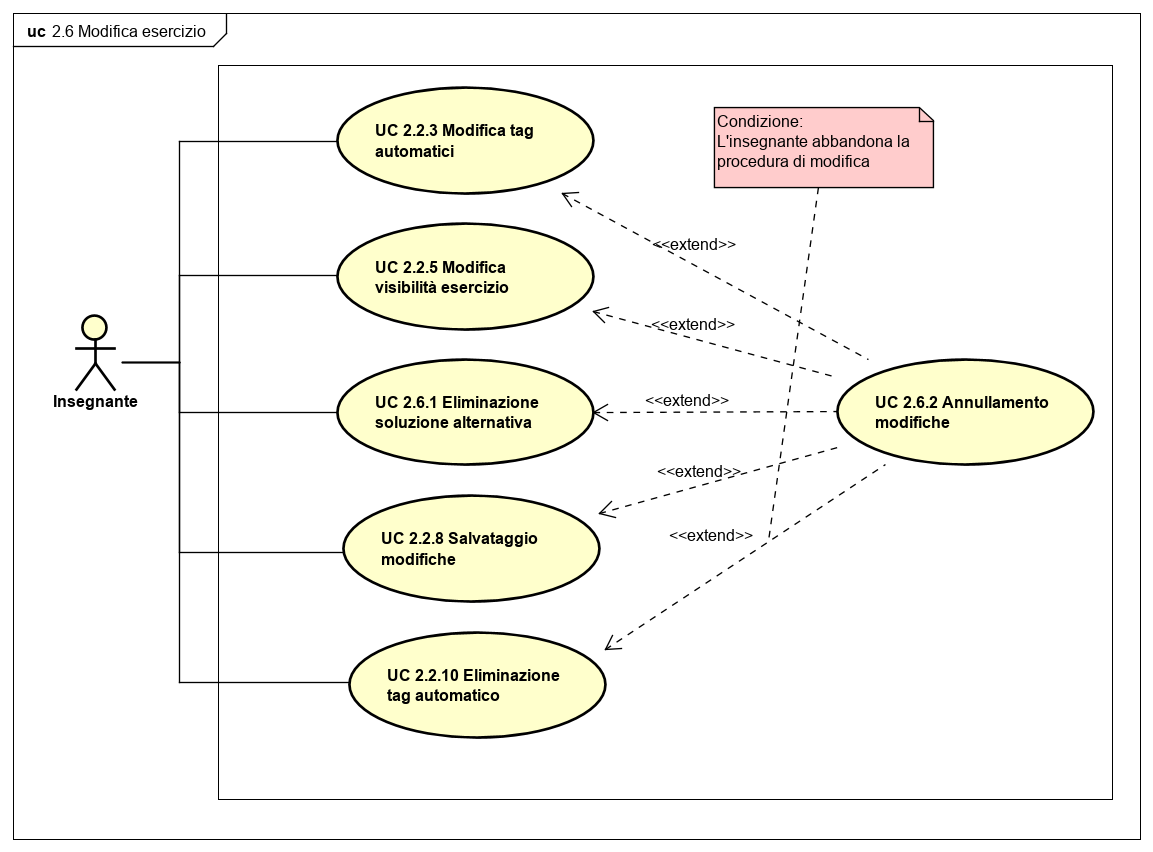
\includegraphics[width=17cm]{img/UC26.png} 
\caption{Caso d'uso UC 2.6}
\end{figure}

\begin{itemize}
	\item[•] \textbf{Attori}: Insegnante;
	\item[•] \textbf{Descrizione}: l’insegnante può modificare il testo, la lingua, la visibilità, i tag e le soluzioni alternative di un esercizio precedentemente inserito;
	\item[•] \textbf{Precondizione}: l'insegnante visualizza lo storico delle frasi inserite;
	\item[•] \textbf{Postcondizione}: l’insegnante ha modificato l'esercizio;
	\item[•] \textbf{Flusso degli eventi}:l’insegnante naviga all’interno della lista degli esercizi inseriti, seleziona un esercizio specifico.
	\item[•] \textbf{Estensioni}
	\begin{enumerate}
		\item UC 2.6.2 Annullamento modifiche.
	\end{enumerate}
\end{itemize}   

\subsubsection{UC 2.6.1 Eliminazione soluzione alternativa}
\begin{itemize}
	\item[•] \textbf{Attori}: Insegnante;
	\item[•] \textbf{Descrizione}: l'insegnante elimina una delle soluzioni alternative inserite in precedenza;
	\item[•] \textbf{Precondizione}: l'insegnante sta modificando un esercizio;
	\item[•] \textbf{Postcondizione}: l'insegnante ha eliminato una soluzione alternativa di un esercizio.
	\item[•] \textbf{Flusso degli eventi}: l'insegnante seleziona apposito campo per l'eliminazione della soluzione alternativa.
\end{itemize}

\subsubsection{UC 2.6.2 Annullamento modifiche}
\begin{itemize}
	\item[•] \textbf{Attori}: Insegnante;
	\item[•] \textbf{Descrizione}: l'insegnante annulla le modifiche inserite all'interno di un esercizio; 
	\item[•] \textbf{Precondizione}: l'insegnante sta modificando un esercizio;
	\item[•] \textbf{Postcondizione}: l'esercizio non è modificato.
	\item[•] \textbf{Flusso degli eventi}:l'insegnante interrompe la procedura di modifica.
\end{itemize}

\subsubsection{UC 2.7 Eliminazione esercizio}
\begin{itemize}
	\item[•] \textbf{Attori}: Insegnante;
	\item[•] \textbf{Descrizione}: l'insegnante ha la possibilità di eliminare un esercizio da lei precedentemente inserito;
	\item[•] \textbf{Precondizione}: l'insegnante visualizza lo storico delle frasi inserite;
	\item[•] \textbf{Postcondizione}: l'insegnante ha eliminato l'esercizio precedentemente inserito;
	\item[•] \textbf{Flusso degli eventi}:l'insegnante seleziona un esercizio specifico e seleziona apposito campo per l'eliminazione.

\subsubsection{UC 2.8 Modifica dati personali}
\begin{itemize}
	\item[•] \textbf{Attori}: Insegnante;
	\item[•] \textbf{Descrizione}: l'insegnante può modificare i propri dati personali;
	\item[•] \textbf{Precondizione}: l'insegnante è stato autenticato dal sistema;
	\item[•] \textbf{Postcondizione}: l'attore interessato ha modificato i propri dati personali;
	\item[•] \textbf{Flusso degli eventi}:
	\begin{enumerate}
		\item UC 2.8.1 Modifico email (sono tutti UC da fare!)
		\item UC 2.8.2 modifico x
		\item UC 2.8.3 modifico y
	\end{enumerate}
\end{itemize}

\subsubsection{UC 2.2.10 Eliminazione tag automatico}
\begin{itemize}
	\item[•] \textbf{Attori}: Insegnante;
	\item[•] \textbf{Descrizione}: l'insegnante elimina uno dei tag automatici generati in precedenza;
	\item[•] \textbf{Precondizione}: l'insegnante sta modificando un esercizio;
	\item[•] \textbf{Postcondizione}: l'insegnante ha eliminato un tag automatico di un esercizio.
	\item[•] \textbf{Flusso degli eventi}: l'insegnante seleziona il tag da eliminare.
\end{itemize}